%\chapter{Ficheros del sistema: el registro} \label{append:registros}

Durante su funcionamiento, \textbf{el limitador genera un registro cada minuto}. El programa encargado de generarlos difiere según la versión, pero en todas ellas se almacenan en el fichero \verb|/var/slr/registro.slr|. Este fichero corresponde en las versiones LM7 y LM9 a un fichero especial de dispositivo de bloques creado mediante la utilidad \verb|mknod|, quedando mapeado\footnote{Crea el fichero \texttt{registro.slr} como un enlace a la partición.} a una partición del disco duro, mientras que en la versión LM11 corresponde a un fichero en formato binario.

El archivo de registros se compone de una cabecera, presente una sola vez al comienzo del fichero, y los registros en sí. El fichero de registro es mantenido por la clase \verb|Registrador|, o \verb|GestorDeRegistro| en la versión LM11, la cual proporciona utilidades para crear, guardar y leer registros. En la figura \ref{fig:lms11-registry-attributes} pueden consultarse los campos que componen la cabecera y cada uno de los registros.

\begin{figure}[h]
	\centering
    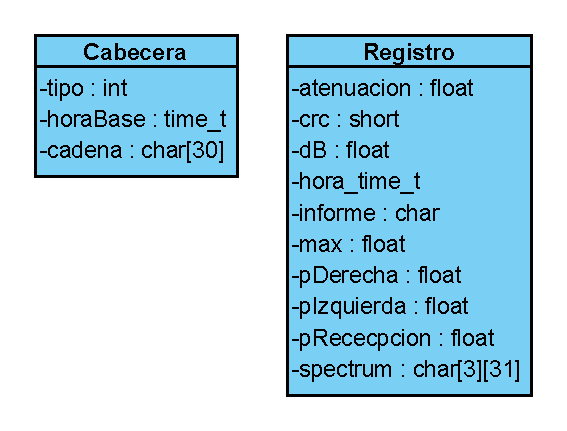
\includegraphics[width=0.55\textwidth]{figuras/lms11-registry-attributes.pdf}
    \caption{Atributos de las clases que componen el registro.}
    \label{fig:lms11-registry-attributes}
\end{figure}